\documentclass[10pt]{beamer}

\usetheme[progressbar=frametitle]{metropolis}
\usepackage{appendixnumberbeamer}

\setbeamertemplate{bibliography item}[text]

\setbeamerfont{bibliography item}{size=\footnotesize}
\setbeamerfont{bibliography entry author}{size=\footnotesize}
\setbeamerfont{bibliography entry title}{size=\footnotesize}
\setbeamerfont{bibliography entry location}{size=\footnotesize}
\setbeamerfont{bibliography entry note}{size=\footnotesize}

\usepackage{array,booktabs}
\usepackage[scale=2]{ccicons}
\usepackage{multicol}
\usepackage{mathtools}
\usepackage{array}

\usepackage{pgfplots}
\usepgfplotslibrary{dateplot}

\usepackage{xspace}

\usepackage{tikz}

\newcommand{\themename}{\textbf{\textsc{metropolis}}\xspace}
\let\oldfootnotesize\footnotesize
\renewcommand*{\footnotesize}{\oldfootnotesize\tiny}
\let\oldabs\abs
\def\abs{\@ifstar{\oldabs}{\oldabs*}}


\title{Introduction to Sentiment Analysis}
\author{Andrew Moore, Paul Rayson}
\date{\today}
\institute{School of Computing and Communications, Lancaster University.}
\titlegraphic{\hfill
\includegraphics[height=1.5cm]{ucrel_logo_2016.png}}

\begin{document}

\maketitle

\begin{frame}{Table of contents}
  \setbeamertemplate{section in toc}[sections numbered]
  \tableofcontents[hideallsubsections]
\end{frame}

\section{Setup}

\begin{frame}{Setup}
\begin{enumerate}
\item Git clone:\\ \url{https://github.com/apmoore1/SentiLexTutorial.git}
\item Within that directory run the following command:\\ \textit{pip3 install -r requirements.txt}
\item Followed by this command:\\ \textit{python3 -m nltk.downloader stopwords}
\end{enumerate}

\end{frame}

\section{Sentiment Analysis Literature}

\begin{frame}[fragile]{What is Sentiment analysis?}
\begin{quote}
is the field of study that analyzes people's opinions, sentiments, appraisals, attitudes, and emotions towards entities and their attributes expressed within text
\end{quote}
\cite{liu2015sentiment}
\end{frame}

\begin{frame}[fragile]{Different levels of sentiment}
\huge
	\begin{columns}[T,onlytextwidth]
      \column{0.4\textwidth}
          \begin{enumerate}
              \setlength\itemsep{2em}
              \item Document
              \item Sentence 
              \item Aspect
          \end{enumerate}
      \column{0.6\textwidth}
          \centering
          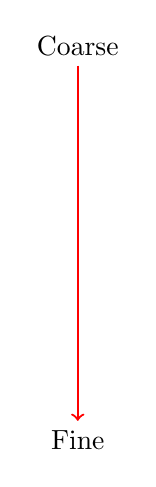
\begin{tikzpicture}
              \node(A){Coarse};
              \node[below of=A, node distance=5cm](B){Fine};
              \path [->, red, thick] (A) edge (B);
          \end{tikzpicture}
	\end{columns}
\end{frame}

\begin{frame}[fragile]{Document sentiment analysis}
  \begin{block}{Objective}
  	To find the sentiment of a document.
  \end{block}
  \begin{block}{Assumption}
    That the document is only discussing one entity
  \end{block}
  \begin{block}{Datasets}
    \begin{enumerate}
      \item Movie Reviews \cite{pang2002,PangSubj04,mass2011}, hotel reviews \cite{wang10}, Amazon reviews \cite{Blitzer07,he16} and restaurant reviews (Yelp)\footnote{\url{https://www.yelp.co.uk/dataset_challenge}}.
      \item Lots of labelled data out there `\textit{in the wild}' and many more datasets that I have missed.
    \end{enumerate}
  \end{block}
\end{frame}

\begin{frame}{Document Example}
  \centering
  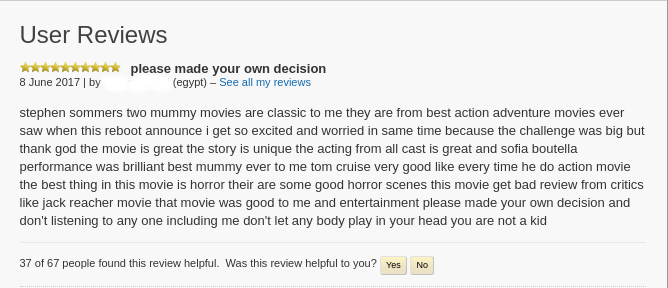
\includegraphics[scale=0.45]{examples/mummy_review.png}\footnote{This came from IDMB website \url{http://www.imdb.com/}}
\end{frame}

\begin{frame}{Document papers to read}
  \huge 
  \begin{enumerate}
    \item Original paper for document and sentiment analysis in general \cite{pang2002}
    \item Unsupervised method \cite{Turney02}
    \item Great evaluation across multiple datasets \cite{Paltoglou10}
    \item New Neural Network (NN) approach \cite{Xu16}
  \end{enumerate}

\end{frame}

\begin{frame}{Sentence sentiment analysis}
  \begin{block}{Objective}
    \begin{enumerate}
      \item To find the sentiment of the sentence.
    \end{enumerate}
  \end{block}
  \begin{block}{Datasets}
    \begin{enumerate}
      \item Movie review sentences \cite{pang05} 
    \end{enumerate}
  \end{block}
  \begin{block}{Papers}
    \begin{enumerate}
      \item One of the original papers \cite{McDonald07}, used a joint model of sentence and document.
      \item Comparisons of different sentence level sentiment classifiers over different datasets \cite{Ribeiro16}
      \item Recusive Neural Network approach RNN \cite{Socher13}
    \end{enumerate}
  \end{block}
  
\end{frame}

\begin{frame}{Sentence Examples}
  \centering
  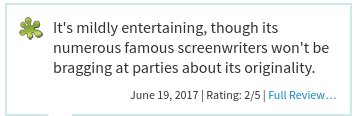
\includegraphics[scale=0.7]{examples/sentence_example.png}\footnote{This came from rotten tomatoes website \url{https://www.rottentomatoes.com}} \\~\\
   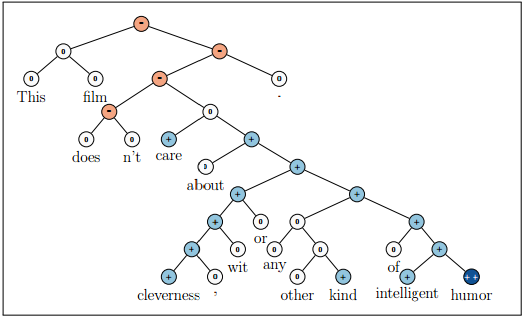
\includegraphics[scale=0.3]{examples/RNTN_example.png}\cite{Socher13}
\end{frame}

\begin{frame}{Subjectivity within sentences}
  \begin{block}{Objective}
    \begin{enumerate}
      \item To determine if the sentence is subjective or objective. 
    \end{enumerate}
  \end{block}
  \begin{block}{Examples}
    \begin{enumerate}
      \item At several different levels, it's a fascinating
tale. Subjective sentence.
      \item Bell Industries Inc. increased its quarterly
to 10 cents from seven cents a share. Objective
sentence. \footnote{Both of these sentences are taken from \cite{Wiebe99}}  
    \end{enumerate}
  \end{block}
  \begin{block}{Datasets}
    \begin{enumerate}
      \item MPQA corpus \cite{Deng15}
      \item Rotten tomatoes dataset \cite{PangSubj04}
    \end{enumerate}
  \end{block}
\end{frame}

\begin{frame}{Subjectivity and uses of subjectivity papers to read}
  \huge
  \begin{enumerate}
    \item Original papers \cite{Wiebe99} and \cite{Riloff03}
    \item Uses subjectivity to show that it is a good summary for document level sentiment analysis \cite{PangSubj04}
  \end{enumerate} 
\end{frame}

\begin{frame}{Twitter Sentiment}
  \begin{block}{Objective}
  Given a Tweet predict the sentiment within it.
  \end{block}
  \begin{block}{Datasets}
    \begin{enumerate}
      \item SemEval Twitter Dataset \cite{Nakov13}
    \end{enumerate}
  \end{block}
  \begin{block}{Metric evaluation}
    \begin{equation}
    F_\text{pos} = \frac{2(p_\text{pos} + r_\text{pos})}{p_\text{pos} * r_\text{pos}}
    \end{equation}
    \begin{equation}
    F = \frac{(F_\text{pos} + F_\text{neg})}{2}
    \end{equation}
  \end{block}
\end{frame}

\begin{frame}{Twitter sentiment papers}
  \begin{enumerate}
    \item Original paper \cite{Pak10} automatically created a training set of Pos, Neg and Objective.
    \item Ensemble approach to Twitter sentiment analysis \cite{Hagen15}
    \item Word embedding approach \cite{Tang14}
  \end{enumerate}

\end{frame}

\begin{frame}{Sentiment lexicons}
  \begin{block}{Objective}
  To create a list of words/phrases that are representative/associated with a sentiment class.
  \end{block}
  \begin{block}{Approaches}
    \begin{enumerate}
      \item Manual - create a sentiment lexicon from scratch by using annotators \cite{Loughran11}.
      \item Thesaurus - expand a known set of sentiment words using relations within a thesaurus e.g. synonym relations \cite{Hu04}
      \item Corpus - created by exploiting co-occurrences within a corpus \cite{Kaji07}
    \end{enumerate}
  \end{block}
  \begin{block}{Other papers}
  Hamilton et al. \cite{Hamilton16} used a word embedding approach to find sentiment words that are domain dependent.
  
  \end{block}
  %\begin{block}{The importance of domain adaptation}
  %Loughran and McDonald \cite{Loughran11} showed the importance of adapting to the finance domain when using there finance specific word list to General Inquirer.
  %\end{block}

\end{frame}

\begin{frame}{Example of corpus lexicon creation}
  \centering
  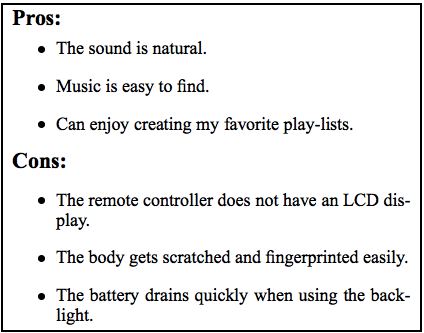
\includegraphics[scale=0.4]{examples/pros_cons.png}\cite{Kaji07}
\end{frame}

\begin{frame}{Aspect}
Aspect sentiment has 7 different properties \cite{ding08,liu2015sentiment}:
\begin{enumerate}
\item Aspect identification.
\item Sentiment of aspect.
\item Aspect groupings.
\item Opinion holder.
\item Time extraction.
\item Sentiment reasoning.
\item Sentiment qualifier.
\end{enumerate}

\end{frame}

\begin{frame}{Aspect Sentiment}
  \begin{block}{Objective}
  Given text identify the sentiment of a specific aspect.
  \end{block}
  \begin{block}{Approaches}
    \begin{enumerate}
      \item Co-occurrences/window frame/pattern/dependencies \cite{Nasukawa03}
      \item Machine learning \cite{Ruder16,Wang16}
    \end{enumerate}
  \end{block}
  \begin{block}{Papers}
    \begin{enumerate}
      \item Original paper \cite{Nasukawa03}
      \item Deep learning \cite{Ruder16}
      \item Deep learning with attention \cite{Wang16}
    \end{enumerate}
  \end{block}
\end{frame}

\begin{frame}{Reproducibility}
Within our area there is a lack of sharing of code. At the moment we are very good at:
\begin{enumerate}
\item Sharing papers
\item Sharing datasets
\end{enumerate}

Unfortunately we are not doing the same with code and this has been noticed \cite{Edison17} 
\end{frame}

\section{Sentiment Workshops}

\begin{frame}{Sentiment analysis workshops}
  \begin{enumerate}
    \item SemEval \footnote{\url{http://alt.qcri.org/semeval2017/}}
    \item WASSA \footnote{\url{http://optima.jrc.it/wassa2017/}}
    \item ESA \footnote{\url{http://gsi.dit.upm.es/esa2016/}}
    \item PEOPLES \footnote{\url{https://peoples2016.github.io/}}
  \end{enumerate}
\end{frame}

\begin{frame}[plain]
\begin{center}
\begin{center}
\huge Questions?
\end{center}
\begin{center}
\begin{columns}[T,onlytextwidth]
\column{0.1\textwidth}
\column{0.4\textwidth}
\centering
Andrew Moore
\\
Paul Rayson
\column{0.4\textwidth}
\centering
@apmoore94
\\
@perayson
\column{0.1\textwidth}
\end{columns}
\end{center}
\end{center}
\end{frame}

\section{Tasks}

\begin{frame}{Task 1: Online sentiment demos}
  \begin{block}{Aim (spend 20 minutes on this, then we'll compare notes)}
  Try out existing web demos to see how they rate your test sentences and how their scores vary. Test them with a variety of capitalisation, repeated letters and exclamation marks for emphasis, plus emoticons. \cite{TehEtAl2016}
  \end{block}
  \begin{block}{Systems}
    \begin{enumerate}
    \item Potts Stanford (7-9 different sentiment lexicons): \url{http://sentiment.christopherpotts.net/textscores/}
    \item SentiStrength: \url{http://sentistrength.wlv.ac.uk/}
    \item NLTK 2.0.4: \url{http://text-processing.com/demo/sentiment/}
    \item TheySay: \url{http://apidemo.theysay.io/}
    \item Daniel Soper: \url{http://www.danielsoper.com/sentimentanalysis/}
    \item LIWC: \url{http://liwc.wpengine.com/}
    \end{enumerate}
  \end{block}

\end{frame}

\begin{frame}{Task 2: Creating your own sentiment lexicon}

We are going to create a sentiment lexicon using word embeddings and a few seed words \cite{Hamilton16}.
\\
~

Go to the Git repository that we cloned at the start in the command line and run the following command:\\
\textit{ipython3 notebook}
\end{frame}

\begin{frame}[allowframebreaks]{References}
  \bibliography{demo}
  \bibliographystyle{abbrv}

\end{frame}

\end{document}
